%% Study pipeline for the LAK/JLA submission -- standalone TikZ.
%% GENERATED by analysis/semantic/oncoco/make_pipeline_tikz.py -- do not edit by hand.
%% Picture-first: each step shows its operation, one short line states its outcome.
\documentclass[border=1pt,10pt]{standalone}
\usepackage[T1]{fontenc}
\usepackage[scaled=0.92]{helvet}
\renewcommand{\familydefault}{\sfdefault}
\usepackage{sansmath}
\sansmath
\usepackage{tikz}
\usetikzlibrary{arrows.meta,positioning,calc}

\definecolor{cReal}{HTML}{2C6E63}
\definecolor{cRP}{HTML}{4A6E9B}
\definecolor{cLLM}{HTML}{C0503C}
\definecolor{cAcc}{HTML}{7A5EA6}
\definecolor{cInk}{HTML}{1F2328}
\definecolor{cMeas}{HTML}{3F4A57}
\definecolor{cMute}{HTML}{70757D}
\definecolor{cRule}{HTML}{CFD4DA}
\definecolor{cPanel}{HTML}{FBFBFC}
\definecolor{cBand}{HTML}{DDE2E8}
\definecolor{cNull}{HTML}{B9C2CC}

\newcommand{\TINY}{\fontsize{4.7}{5.4}\selectfont}
\newcommand{\MICRO}{\fontsize{5.2}{6.0}\selectfont}

% #1 x0  #2 y0  #3 width  #4 height  #5 number  #6 title
\newcommand{\stepbox}[6]{%
  \draw[rounded corners=2.5pt, draw=cRule, fill=cPanel, line width=0.5pt,
        dash pattern=on 2.2pt off 1.6pt] (#1,#2) rectangle (#1+#3,#2+#4);
  \node[circle, fill=cInk, text=white, inner sep=0pt, minimum size=3.2mm,
        font=\bfseries\fontsize{5.6}{6.6}\selectfont] at (#1+0.36,#2+#4-0.38) {#5};
  \node[anchor=west, font=\scriptsize\bfseries, text=cInk, inner sep=0pt]
       at (#1+0.58,#2+#4-0.38) {#6};
}
% #1 x0  #2 y0  #3 width  #4 accent colour  #5 one-line outcome
\newcommand{\outcome}[5]{%
  \fill[#4!8, rounded corners=1.6pt] (#1+0.16,#2) rectangle (#1+#3-0.16,#2+0.46);
  \draw[#4, line width=0.9pt] (#1+0.16,#2) -- (#1+0.16,#2+0.46);
  \node[anchor=west, font=\MICRO\bfseries, text=#4, inner sep=0pt] at (#1+0.30,#2+0.23) {#5};
}
% #1 x  #2 y  #3 text
\newcommand{\ann}[3]{%
  \node[anchor=north west, font=\TINY, text=cMute, align=left, text width=2.80cm,
        inner sep=0pt] at (#1,#2) {#3};
}

\begin{document}
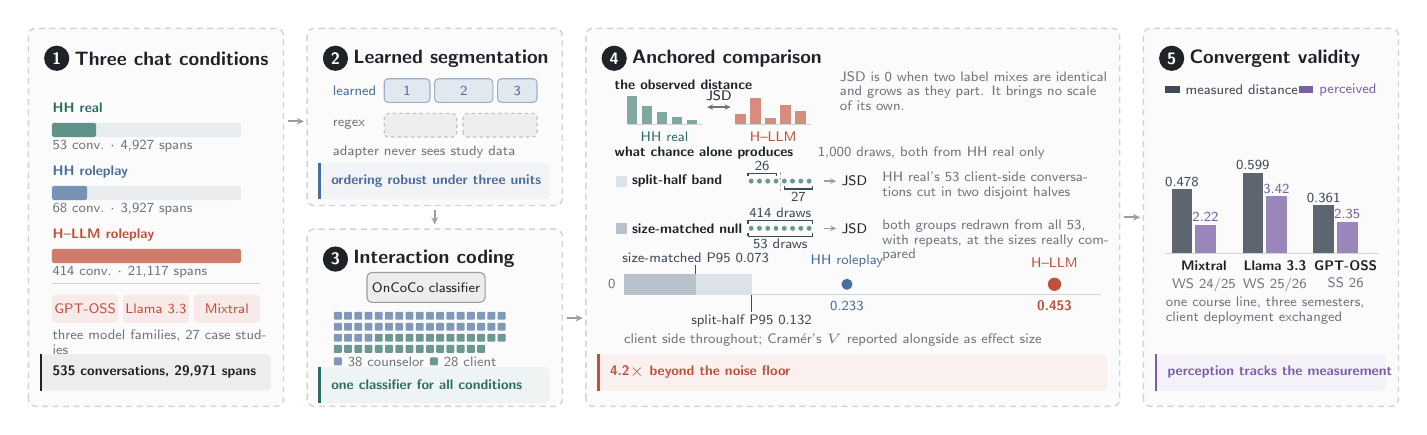
\begin{tikzpicture}[x=1cm,y=1cm]
\path (0,0) rectangle (17.40,4.80);

\draw[-{Stealth[length=2.6pt,width=2.4pt]}, cMute!70, line width=0.8pt] (3.30,3.62) -- (3.50,3.62);
\draw[-{Stealth[length=2.6pt,width=2.4pt]}, cMute!70, line width=0.8pt] (5.16,2.49) -- (5.16,2.31);
\draw[-{Stealth[length=2.6pt,width=2.4pt]}, cMute!70, line width=0.8pt] (6.84,1.12) -- (7.04,1.12);
\draw[-{Stealth[length=2.6pt,width=2.4pt]}, cMute!70, line width=0.8pt] (13.92,2.40) -- (14.12,2.40);

%% ================================================= 1  three chat corpora
\stepbox{0.00}{0.00}{3.24}{4.80}{1}{Three chat conditions}

% each row: name, a span bar drawn to scale, the counts
\foreach \y/\c/\name/\w/\meta in {%
  3.86/cReal/HH real/0.560/53 conv.\ $\cdot$ 4{,}927 spans,
  3.06/cRP/HH roleplay/0.446/68 conv.\ $\cdot$ 3{,}927 spans,
  2.26/cLLM/H--LLM roleplay/2.400/414 conv.\ $\cdot$ 21{,}117 spans}{
  \node[anchor=north west, font=\MICRO\bfseries, text=\c, inner sep=0pt]
       at (0.30,\y) {\name};
  \fill[cRule!45, rounded corners=0.8pt] (0.30,\y-0.44) rectangle (2.70,\y-0.26);
  \fill[\c!75, rounded corners=0.8pt] (0.30,\y-0.44) rectangle (0.30+\w,\y-0.26);
  \ann{0.30}{\y-0.48}{\meta}
}
\draw[cRule, line width=0.4pt] (0.30,1.56) -- (2.94,1.56);
\foreach \i/\m in {0/GPT-OSS, 1/Llama 3.3, 2/Mixtral}{
  \pgfmathsetmacro{\xa}{0.30 + \i*0.90}
  \fill[cLLM!12, rounded corners=1.4pt] (\xa,1.06) rectangle (\xa+0.84,1.42);
  \node[anchor=center, font=\TINY, text=cLLM, inner sep=0pt] at (\xa+0.42,1.24) {\m};
}
\ann{0.30}{0.98}{three model families, 27 case studies}
\outcome{0.00}{0.20}{3.24}{cInk}{535 conversations, 29{,}971 spans}

%% ================================================= 2  learned segmentation
\stepbox{3.54}{2.55}{3.24}{2.25}{2}{Learned segmentation}

\node[anchor=west, font=\TINY, text=cRP, inner sep=0pt] at (3.86,4.01) {learned};
\foreach \xa/\w/\lab in {4.52/0.58/1, 5.16/0.74/2, 5.96/0.50/3}{
  \fill[cRP!16, rounded corners=1.4pt] (\xa,3.86) rectangle (\xa+\w,4.16);
  \draw[cRP!55, line width=0.4pt, rounded corners=1.4pt] (\xa,3.86) rectangle (\xa+\w,4.16);
  \node[anchor=center, font=\TINY, text=cRP, inner sep=0pt] at (\xa+\w/2,4.01) {\lab};
}
\node[anchor=west, font=\TINY, text=cMute, inner sep=0pt] at (3.86,3.57) {regex};
\foreach \xa/\w in {4.52/0.92, 5.52/0.94}{
  \fill[cMute!12, rounded corners=1.4pt] (\xa,3.42) rectangle (\xa+\w,3.72);
  \draw[cMute!45, line width=0.4pt, dash pattern=on 1.2pt off 1.2pt, rounded corners=1.4pt]
       (\xa,3.42) rectangle (\xa+\w,3.72);
}
\ann{3.86}{3.32}{adapter never sees study data}
\outcome{3.54}{2.63}{3.24}{cRP}{ordering robust under three units}

%% ================================================= 3  interaction coding
\stepbox{3.54}{0.00}{3.24}{2.25}{3}{Interaction coding}

\fill[cInk!8, rounded corners=1.8pt] (4.30,1.32) rectangle (5.80,1.70);
\draw[cInk!45, line width=0.4pt, rounded corners=1.8pt] (4.30,1.32) rectangle (5.80,1.70);
\node[anchor=center, font=\TINY, text=cInk, inner sep=0pt] at (5.05,1.51) {OnCoCo classifier};

% the label inventory, one cell per category (38 counselor + 28 client = the
% published 66-category scheme; a fixed property of the instrument, not a result)
\foreach \i in {0,...,65}{
  \pgfmathsetmacro{\col}{mod(\i,17)}
  \pgfmathsetmacro{\row}{floor(\i/17)}
  \pgfmathsetmacro{\xa}{3.88 + \col*0.13}
  \pgfmathsetmacro{\ya}{1.10 - \row*0.14}
  \ifnum\i<38
    \fill[cRP!70, rounded corners=0.3pt] (\xa,\ya) rectangle (\xa+0.10,\ya+0.10);
  \else
    \fill[cReal!70, rounded corners=0.3pt] (\xa,\ya) rectangle (\xa+0.10,\ya+0.10);
  \fi
}
\fill[cRP!70, rounded corners=0.3pt] (3.88,0.52) rectangle (3.98,0.62);
\node[anchor=west, font=\TINY, text=cMute, inner sep=0pt] at (4.05,0.57) {38 counselor};
\fill[cReal!70, rounded corners=0.3pt] (5.10,0.52) rectangle (5.20,0.62);
\node[anchor=west, font=\TINY, text=cMute, inner sep=0pt] at (5.27,0.57) {28 client};
\outcome{3.54}{0.04}{3.24}{cReal}{one classifier for all conditions}

%% ================================================= 4  anchored comparison
%% Three stacked rows: what is measured, how the two nulls are built, and the
%% ruler both are read on. The null constructions are drawn as mechanics --
%% disjoint brackets for the split-half band, full-span brackets for the
%% size-matched null -- because that contrast is the whole point of having two.
\stepbox{7.08}{0.00}{6.78}{4.80}{4}{Anchored comparison}

%% ---- row 1: what is measured -----------------------------------------
\node[anchor=west, font=\MICRO\bfseries, text=cInk, inner sep=0pt] at (7.44,4.08) {the observed distance};
\foreach \i/\h in {0/0.36, 1/0.24, 2/0.16, 3/0.10, 4/0.06}{
  \pgfmathsetmacro{\xa}{7.60 + \i*0.19}
  \fill[cReal!60] (\xa,3.58) rectangle (\xa+0.13,3.58+\h);
}
\foreach \i/\h in {0/0.13, 1/0.33, 2/0.08, 3/0.25, 4/0.17}{
  \pgfmathsetmacro{\xa}{8.98 + \i*0.19}
  \fill[cLLM!65] (\xa,3.58) rectangle (\xa+0.13,3.58+\h);
}
\draw[cRule, line width=0.4pt] (7.60,3.58) -- (8.56,3.58);
\draw[cRule, line width=0.4pt] (8.98,3.58) -- (9.94,3.58);
\node[anchor=north, font=\TINY, text=cReal, inner sep=1.2pt] at (8.08,3.54) {HH real};
\node[anchor=north, font=\TINY, text=cLLM, inner sep=1.2pt] at (9.46,3.54) {H--LLM};
\draw[{Stealth[length=2.2pt,width=2.0pt]}-{Stealth[length=2.2pt,width=2.0pt]},
      cMute, line width=0.5pt] (8.62,3.80) -- (8.92,3.80);
\node[anchor=south, font=\TINY, text=cInk, inner sep=1.0pt] at (8.77,3.84) {JSD};
\node[anchor=north west, font=\TINY, text=cMute, align=left, text width=3.44cm, inner sep=0pt]
     at (10.30,4.26) {JSD is 0 when two label mixes are identical and grows as they part. It brings no scale of its own.};

%% ---- row 2: how the two nulls are built ------------------------------
\node[anchor=west, font=\MICRO\bfseries, text=cInk, inner sep=0pt] at (7.44,3.22) {what chance alone produces};
\node[anchor=west, font=\TINY, text=cMute, inner sep=0pt] at (10.02,3.22) {1{,}000 draws, both from HH real only};

% split-half band: the reference cut in two, every conversation on one side
\fill[cBand] (7.46,2.79) rectangle (7.60,2.93);
\node[anchor=west, font=\TINY\bfseries, text=cInk, inner sep=0pt] at (7.66,2.86) {split-half band};
\foreach \i in {0,...,7}{
  \pgfmathsetmacro{\xa}{9.18 + \i*0.105}
  \fill[cReal!70] (\xa,2.86) circle (0.9pt);
}
\draw[cMute!60, line width=0.35pt, dash pattern=on 1.0pt off 1.0pt] (9.55,2.73) -- (9.55,2.99);
\draw[cMeas, line width=0.5pt] (9.14,2.96) -- (9.50,2.96);
\draw[cMeas, line width=0.5pt] (9.14,2.96) -- (9.14,2.92);
\draw[cMeas, line width=0.5pt] (9.50,2.96) -- (9.50,2.92);
\node[anchor=south, font=\TINY, text=cMeas, inner sep=0.6pt] at (9.32,2.97) {26};
\draw[cMeas, line width=0.5pt] (9.60,2.76) -- (9.96,2.76);
\draw[cMeas, line width=0.5pt] (9.60,2.76) -- (9.60,2.80);
\draw[cMeas, line width=0.5pt] (9.96,2.76) -- (9.96,2.80);
\node[anchor=north, font=\TINY, text=cMeas, inner sep=0.6pt] at (9.78,2.75) {27};
\draw[-{Stealth[length=2.2pt,width=2.0pt]}, cMute!70, line width=0.6pt] (10.10,2.86) -- (10.26,2.86);
\node[anchor=west, font=\TINY, text=cInk, inner sep=0pt] at (10.32,2.86) {JSD};
\node[anchor=north west, font=\TINY, text=cMute, align=left, text width=2.92cm, inner sep=0pt]
     at (10.84,2.98) {HH real's 53 client-side conversations cut in two disjoint halves};

% size-matched null: both groups redrawn from the whole reference, with repeats
\fill[cNull] (7.46,2.19) rectangle (7.60,2.33);
\node[anchor=west, font=\TINY\bfseries, text=cInk, inner sep=0pt] at (7.66,2.26) {size-matched null};
\foreach \i in {0,...,7}{
  \pgfmathsetmacro{\xa}{9.18 + \i*0.105}
  \fill[cReal!70] (\xa,2.26) circle (0.9pt);
}
\draw[cMeas, line width=0.5pt] (9.14,2.36) -- (9.96,2.36);
\draw[cMeas, line width=0.5pt] (9.14,2.36) -- (9.14,2.32);
\draw[cMeas, line width=0.5pt] (9.96,2.36) -- (9.96,2.32);
\node[anchor=south, font=\TINY, text=cMeas, inner sep=0.6pt] at (9.55,2.37) {414 draws};
\draw[cMeas, line width=0.5pt] (9.14,2.16) -- (9.96,2.16);
\draw[cMeas, line width=0.5pt] (9.14,2.16) -- (9.14,2.20);
\draw[cMeas, line width=0.5pt] (9.96,2.16) -- (9.96,2.20);
\node[anchor=north, font=\TINY, text=cMeas, inner sep=0.6pt] at (9.55,2.15) {53 draws};
\draw[-{Stealth[length=2.2pt,width=2.0pt]}, cMute!70, line width=0.6pt] (10.10,2.26) -- (10.26,2.26);
\node[anchor=west, font=\TINY, text=cInk, inner sep=0pt] at (10.32,2.26) {JSD};
\node[anchor=north west, font=\TINY, text=cMute, align=left, text width=2.92cm, inner sep=0pt]
     at (10.84,2.38) {both groups redrawn from all 53, with repeats, at the sizes really compared};

%% ---- row 3: the ruler both nulls calibrate ---------------------------
% client side, 12.0 cm per JSD unit; shaded bars run from 0 to each P95
\draw[cRule, line width=0.4pt] (7.56,1.42) -- (13.62,1.42);
\fill[cBand] (7.56,1.42) rectangle (9.184,1.68);
\fill[cNull] (7.56,1.42) rectangle (8.475,1.68);
\fill[cRP] (10.396,1.55) circle (2.0pt);
\fill[cLLM] (13.032,1.55) circle (2.4pt);
\node[anchor=south, font=\TINY, text=cRP, inner sep=1.6pt] at (10.396,1.70) {HH roleplay};
\node[anchor=south, font=\TINY, text=cLLM, inner sep=1.6pt] at (13.032,1.70) {H--LLM};
\node[anchor=north, font=\TINY, text=cRP, inner sep=1.6pt] at (10.396,1.40) {0.233};
\node[anchor=north, font=\TINY\bfseries, text=cLLM, inner sep=1.6pt] at (13.032,1.40) {0.453};
\node[anchor=east, font=\TINY, text=cMute, inner sep=1.6pt] at (7.52,1.55) {0};
\draw[cMeas, line width=0.5pt] (8.475,1.68) -- (8.475,1.79);
\node[anchor=south, font=\TINY, text=cMeas, inner sep=0.6pt] at (8.475,1.80) {size-matched P95 0.073};
\draw[cMeas, line width=0.5pt] (9.184,1.42) -- (9.184,1.20);
\node[anchor=north, font=\TINY, text=cMeas, inner sep=0.6pt] at (9.184,1.19) {split-half P95 0.132};

\node[anchor=west, font=\TINY, text=cMute, inner sep=0pt] at (7.56,0.84) {client side throughout; Cram\'er's $V$ reported alongside as effect size};
\outcome{7.08}{0.20}{6.78}{cLLM}{4.2$\times$ beyond the noise floor}

%% ================================================= 5  convergent validity
\stepbox{14.16}{0.00}{3.24}{4.80}{5}{Convergent validity}

\draw[cMeas, line width=2.4pt] (14.44,4.02) -- (14.62,4.02);
\node[anchor=west, font=\TINY, text=cMeas, inner sep=0pt] at (14.69,4.02) {measured distance};
\draw[cAcc, line width=2.4pt] (16.14,4.02) -- (16.32,4.02);
\node[anchor=west, font=\TINY, text=cAcc, inner sep=0pt] at (16.39,4.02) {perceived};

\foreach \i/\j/\r/\m in {0/0.478/2.22/{Mixtral}, 1/0.599/3.42/{Llama 3.3}, 2/0.361/2.35/{GPT-OSS}}{
  \pgfmathsetmacro{\xa}{14.52 + \i*0.90}
  \pgfmathsetmacro{\hj}{\j/0.7*1.2}
  \pgfmathsetmacro{\hr}{(\r-1)/4*1.2}
  \fill[cMeas!85] (\xa,1.94) rectangle (\xa+0.26,1.94+\hj);
  \fill[cAcc!75] (\xa+0.30,1.94) rectangle (\xa+0.56,1.94+\hr);
  \node[anchor=south, font=\TINY, text=cMeas, inner sep=0.8pt] at (\xa+0.13,1.94+\hj) {\j};
  \node[anchor=south, font=\TINY, text=cAcc, inner sep=0.8pt] at (\xa+0.43,1.94+\hr) {\r};
  \node[anchor=north, font=\TINY\bfseries, text=cInk, inner sep=1.4pt] at (\xa+0.41,1.90) {\m};
}
\draw[cRule, line width=0.4pt] (14.44,1.94) -- (17.14,1.94);
\node[anchor=north, font=\TINY, text=cMute, inner sep=1.2pt] at (14.93,1.68) {WS 24/25};
\node[anchor=north, font=\TINY, text=cMute, inner sep=1.2pt] at (15.83,1.68) {WS 25/26};
\node[anchor=north, font=\TINY, text=cMute, inner sep=1.2pt] at (16.73,1.68) {SS 26};
\ann{14.44}{1.40}{one course line, three semesters, client deployment exchanged}
\outcome{14.16}{0.20}{3.24}{cAcc}{perception tracks the measurement}

\end{tikzpicture}
\end{document}
